\section{Methods}

\begin{comment}
\subsection{Approach}

\subsubsection{Probabilistic modeling based on fundamental statistical analysis of data and priors}

To solve the problems with existing CoSMoS data analysis methods identified above, we have developed a new image-analysis-based approach that is accurate, objective, and built on a rigorous statistical approach to the CoSMoS image analysis problem. This method is based on probabilistic modeling methodology. Bayesian model is a statistical model where probability is used to represent all uncertainty within the model, both for observed and hidden quantities in a system of interest. Bayes' theorem allows to perform inference on hidden variables given the observed data. The method described here is time-independent meaning that we ignore the time dimension of the recording -- the order of the images is arbitrary and does not affect the model, as each image is considered statistically independent of the others. We note that this time-independent method can naturally be extended into a time-dependent approach to both more accurately analyze the images and to directly obtain information about molecular kinetic mechanisms.  The proposed methods will eliminate the need for subjective image inspection and minimize the manual work required for CoSMoS data analysis. 

Unlike standard analysis methods for CoSMoS and single molecule FRET (smFRET), which are based on scalar intensity measurements derived from integration of emission in image regions of interest, our model fully uses information contained in the raw two-dimensional microscope images. The value of image data is proven in previous studies \citep{Friedman2015-nx,Smith2019-yb}. To analyze the CoSMoS image classification problem within a Bayesian framework, one must define ideal image shapes for each class (image model) and choose a likelihood function for the observed data (noise model).
\end{comment}

The images are diffraction-limited point spread functions. CoSMoS images consist of background intensity and diffraction-limited spots. The CoSMoS data set consists of a set of images where we have $N$ target sites ($n \in \{1,\dots,N\}$) each consisting of a series of $F$ different images in a recording ($f \in \{1,\dots,F\}$) (a “recording”). Each image is represented as a matrix (2D-array) of $P \times P$ pixel intensities ($i,j \in \{1,\dots,P\}$). We denote entire data set as a multi-dimensional array $D$ and the value of a specific pixel intensity as $D_{nfij}$.

Our goal is to extract useful information from the data such as the probability of the presence of the on-target molecule. Our approach is to use statistical modeling. We formulate a generative model that describes how the observed data is produced. Then we make inference on latent variables that describe the physical parameters of the generative model. 

\subsection{Model}

We build a probabilistic model for CoSMoS data by introducing latent variables that explain how the observed data is generated. A graphical model describing the probabilistic relationships in the model is shown in Figure \ref{fig:graph}. In this directed graph, nodes are either random variables (circles) or deterministic functions (diamonds). Related nodes are connected by edges, with an arrow pointing towards the dependent variable. Dashed boxes represent activation of variables. Finally, plates represent replication and specify an index for the repeated variable.

\begin{figure}[ht]
  \begin{center}
    % model_pca2.tex
%
% Copyright (C) 2010,2011 Laura Dietz
% Copyright (C) 2012 Jaakko Luttinen
%
% The MIT License
%
% See LICENSE file for more details.

% PCA model

%\beginpgfgraphicnamed{model-pca}
\begin{tikzpicture}

  % Define nodes

  % Y
  \node[obs]          (D)   {$D$}; %

  % W and X
  \node[det, above=of D]            (md) {$\mu^D$} ; % 
  \node[latent, above=of md] (w)   {$w$}; %
  \node[latent, above=of md, left=of w]  (h)   {$h$}; %
  \node[latent, above=of md, left=of h]  (b)   {$b$}; %
  \node[latent, above=of md, right=of w]  (x)   {$x$}; %
  \node[latent, above=of md, right=of x] (y)   {$y$}; %

  % b hyperparameters
  \node[const, above=2.8 of b, xshift=-0.5cm] (mb) {$\mu^b$} ; %
  \node[const, above=3.5 of b, xshift=0.5cm]  (bb) {$\beta^b$} ; %

  % h hyperparameters
  \node[const, above=3.5 of h, xshift=-0.5cm] (mh) {$\mu^h$} ; %
  \node[const, above=3.5 of h, xshift=0.5cm]  (bh) {$\beta^h$} ; %

  % w hyperparameters
  \node[const, above=3.5 of w, xshift=-0.5cm] (mw) {$\mu^w$} ; %
  \node[const, above=3.5 of w, xshift=0.5cm]  (nw) {$\nu^w$} ; %

  % xy hyperparameters
  \node[const, above=3.5 of x, xshift=-0.1cm] (mxy) {$\mu^{x,y}=0$} ; %
  \node[const, above=3.5 of y, xshift=0.1cm] (pr) {$\nu_{flat},\nu_{prox}$} ; %
  \node[det, above=1.4 of y]  (nxy) {$\nu^{x,y}$} ; %

  % Factors
  \factor[above=of D] {D-f} {left:$\mathcal{G}$} {} {} ; %
  \factor[above=0.6 of b] {b-f} {left:$\mathcal{G}$} {mb,bb} {b} ; %
  \factor[above=0.6 of h] {h-f} {left:$\mathcal{G}$} {mh,bh} {h} ; %
  \factor[above=0.6 of w] {w-f} {left:$\mathcal{B}$} {mw,nw} {w} ; %
  \factor[above=0.6 of x] {x-f} {left:$\mathcal{B}$} {mxy,nxy} {x} ; %
  \factor[above=0.6 of y] {y-f} {left:$\mathcal{B}$} {mxy,nxy} {y} ; %

  % D hyperparameters
  \node[const, right=8 of D-f] (g) {gain} ; %

  % m and theta
  \node[latent, right=of y-f] (m)   {$m$}; %
  \node[latent, above=0.5 of m] (t)   {$\theta$}; %

  % m and theta hyperparameters
  \node[det, right=1. of m]        (pm) {$\pi^m$} ; %
  \node[det, right=1. of t]        (pt) {$\pi^\theta$} ; %
  \node[const, right=of pt] (pz) {$\pi^z$} ; %
  \node[const, right=of pm] (lj) {$\lambda^j$} ; %

  % theta hyperparameters
  %\node[const, right=1.2 of t] (pt) {$\pi^\theta(\pi^z,\lambda^j)$} ; %

  % noise
  %\node[latent, right=2.5cm of y-f]         (t)   {$\tau$}; %
  %\node[const, above=of t, xshift=-0.5cm] (at)  {$\alpha_\tau$} ; %
  %\node[const, above=of t, xshift=0.5cm]  (bt)  {$\beta_\tau$} ; %

  % Factors
  \factor[right=of m] {m-f} {above:$\mathcal{C}$} {pm} {m} ; %
  \factor[right=of t] {t-f} {above:$\mathcal{C}$} {pt} {t} ; %
  %\factor[above=of x] {x-f} {left:$\mathcal{N}$} {mx,ax} {x} ; %
  %\factor[above=of t] {t-f} {left:$\mathcal{G}$} {at,bt} {t} ; %
  %\factoredge {dot,t} {y-f} {y} ; %

  \gate {m-gate} {(h-f)(h-f-caption)(h-f)(h-f-caption)(w-f)(w-f-caption)(x-f)(x-f-caption)(y-f)(y-f-caption)} {m}

  % Connect w and x to the dot node
  \factoredge[-] {g,md} {D-f} {D} ;
  \edge[-] {b,h,w,x,y} {md} ;
  \edge[-] {pz} {pt} ;
  \edge[-] {lj,t} {pm} ;
  \edge[-] {t,pr} {nxy} ;

  % Plates
  \plate {K} { %
    (h)(h-f)(h-f-caption) %
    (w)(w-f)(w-f-caption) %
    (x)(x-f)(x-f-caption) %
    (y)(y-f)(y-f-caption) %
    (m-gate) %
    (nxy)
  } {$\forall k \in \{ 1..K \}$} ;
  \plate {F} { %
    (K)
    (t)(t-f)(t-f-caption)(pt) %
    (m)(m-f)(m-f-caption)(pm) %
    (b)(b-f)(b-f-caption) %
    (md) %
    (D)(D-f)(D-f-caption) %
  } {$\forall f \in \{ 1..F \}$} ;
  \plate {N} { %
    (F)
    (mb)
  } {$\forall n \in \{ 1..N \}$} ;
  %\plate {} {%
    %(y)(y-f)(y-f-caption) %
    %(w)(w-f)(w-f-caption) %
    %(dot) %
    %(yx.north west)(yx.south west) %
  %} {$M$} ;

\end{tikzpicture}
%\endpgfgraphicnamed

%%% Local Variables: 
%%% mode: tex-pdf
%%% TeX-master: "example"
%%% End: 


  \end{center}
  \caption{Graphical model for the Bayesian classification model used in Pyro. The model has a modular structure consisting of three parts: classifier, the spot model, and the noise model. Hidden variables (circles) - background intensity ($b$), integrated intensity of the spot ($h$), width of the spot ($w$), position of the spot on the $x$-axis ($x$) and on the $y$-axis ($y$), existence indicator of spots ($m$), and index of the on-target spot ($\theta$). Observed variable (shaded circle) - image of the area of interest ($D$). Variables nested in plates are repeated for a number of times displayed at the bottom-right corner - target sites ($N$), frame count ($F$), number of spots in a single image ($K$). Densities are depicted as  small filled boxes. Deterministic functions are depicted as diamonds. Constants and hyperparameters are written without any borders. Gate (dashed box) represents variable activation conditioned on another variable.}
  \label{fig:graph}
\end{figure}

\subsubsection{Physical model}

We model the observed image data as ``spot'' images of binder molecules superimposed on background image. In particular, background image consists only of constant background intensity $\mathrm{b}_{nf}$ that can vary from image to image. Our model assumes that at maximum $K$ number of spots can be present in a single image.  Fluorescence spot is modeled as a 2D Gaussian which accurately approximates fluorescence microscope point spread function \citep{Zhang2007-rb}. Each spot is parameterized by integrated scalar intensity $\mathrm{h}_{nfk}$, width $\mathrm{w}_{nfk}$, and positions $\mathrm{x}_{nfk}$ and $\mathrm{y}_{nfk}$ on the image:

\begin{equation}
    \mu^{S}_{nfkij} =
        \dfrac{\mathrm{h}_{nfk}}{2 \pi \mathrm{w}^2_{nfk}} \exp{\left[ -\dfrac{(i-\mathbf{x}_{nfk})^2 + (j-\mathrm{y}_{nfk})^2}{2\mathrm{w}^2_{nfk}} \right]}
\end{equation}

We use binary indicator variable $\mathbf{m} = \{\mathrm{m}_{nfk}\}$ to denote the presence of each individual spot ($k \in \{1,\dots,K\}$). The value of the index variable $\theta_{nf} \in \{0,1,\dots,K\}$ specifies the index of the on-target spot when it is present and equals zero when the on-target spot is absent. There are $2^K + K2^{K-1}$ unique combinations of $\mathrm{m}$ and $\theta$ which define the state space for each image. Table~\ref{tab:states} shows the state space when $K=2$.

Thus, we get the image model ($\mu^I_{nfij}$) calculated as the sum of the background intensity ($\mathrm{b}_{nf}$) and 2D Gaussian spots ($\mu^S_{knfij}$) present in the image:

\begin{equation}
    \mu^\mathrm{I}_{nfij} = \mathrm{b}_{nf} + \sum_{\mathrm{m}_{nfk}=1} \mu^S_{knfij}
\end{equation}

\begin{figure}
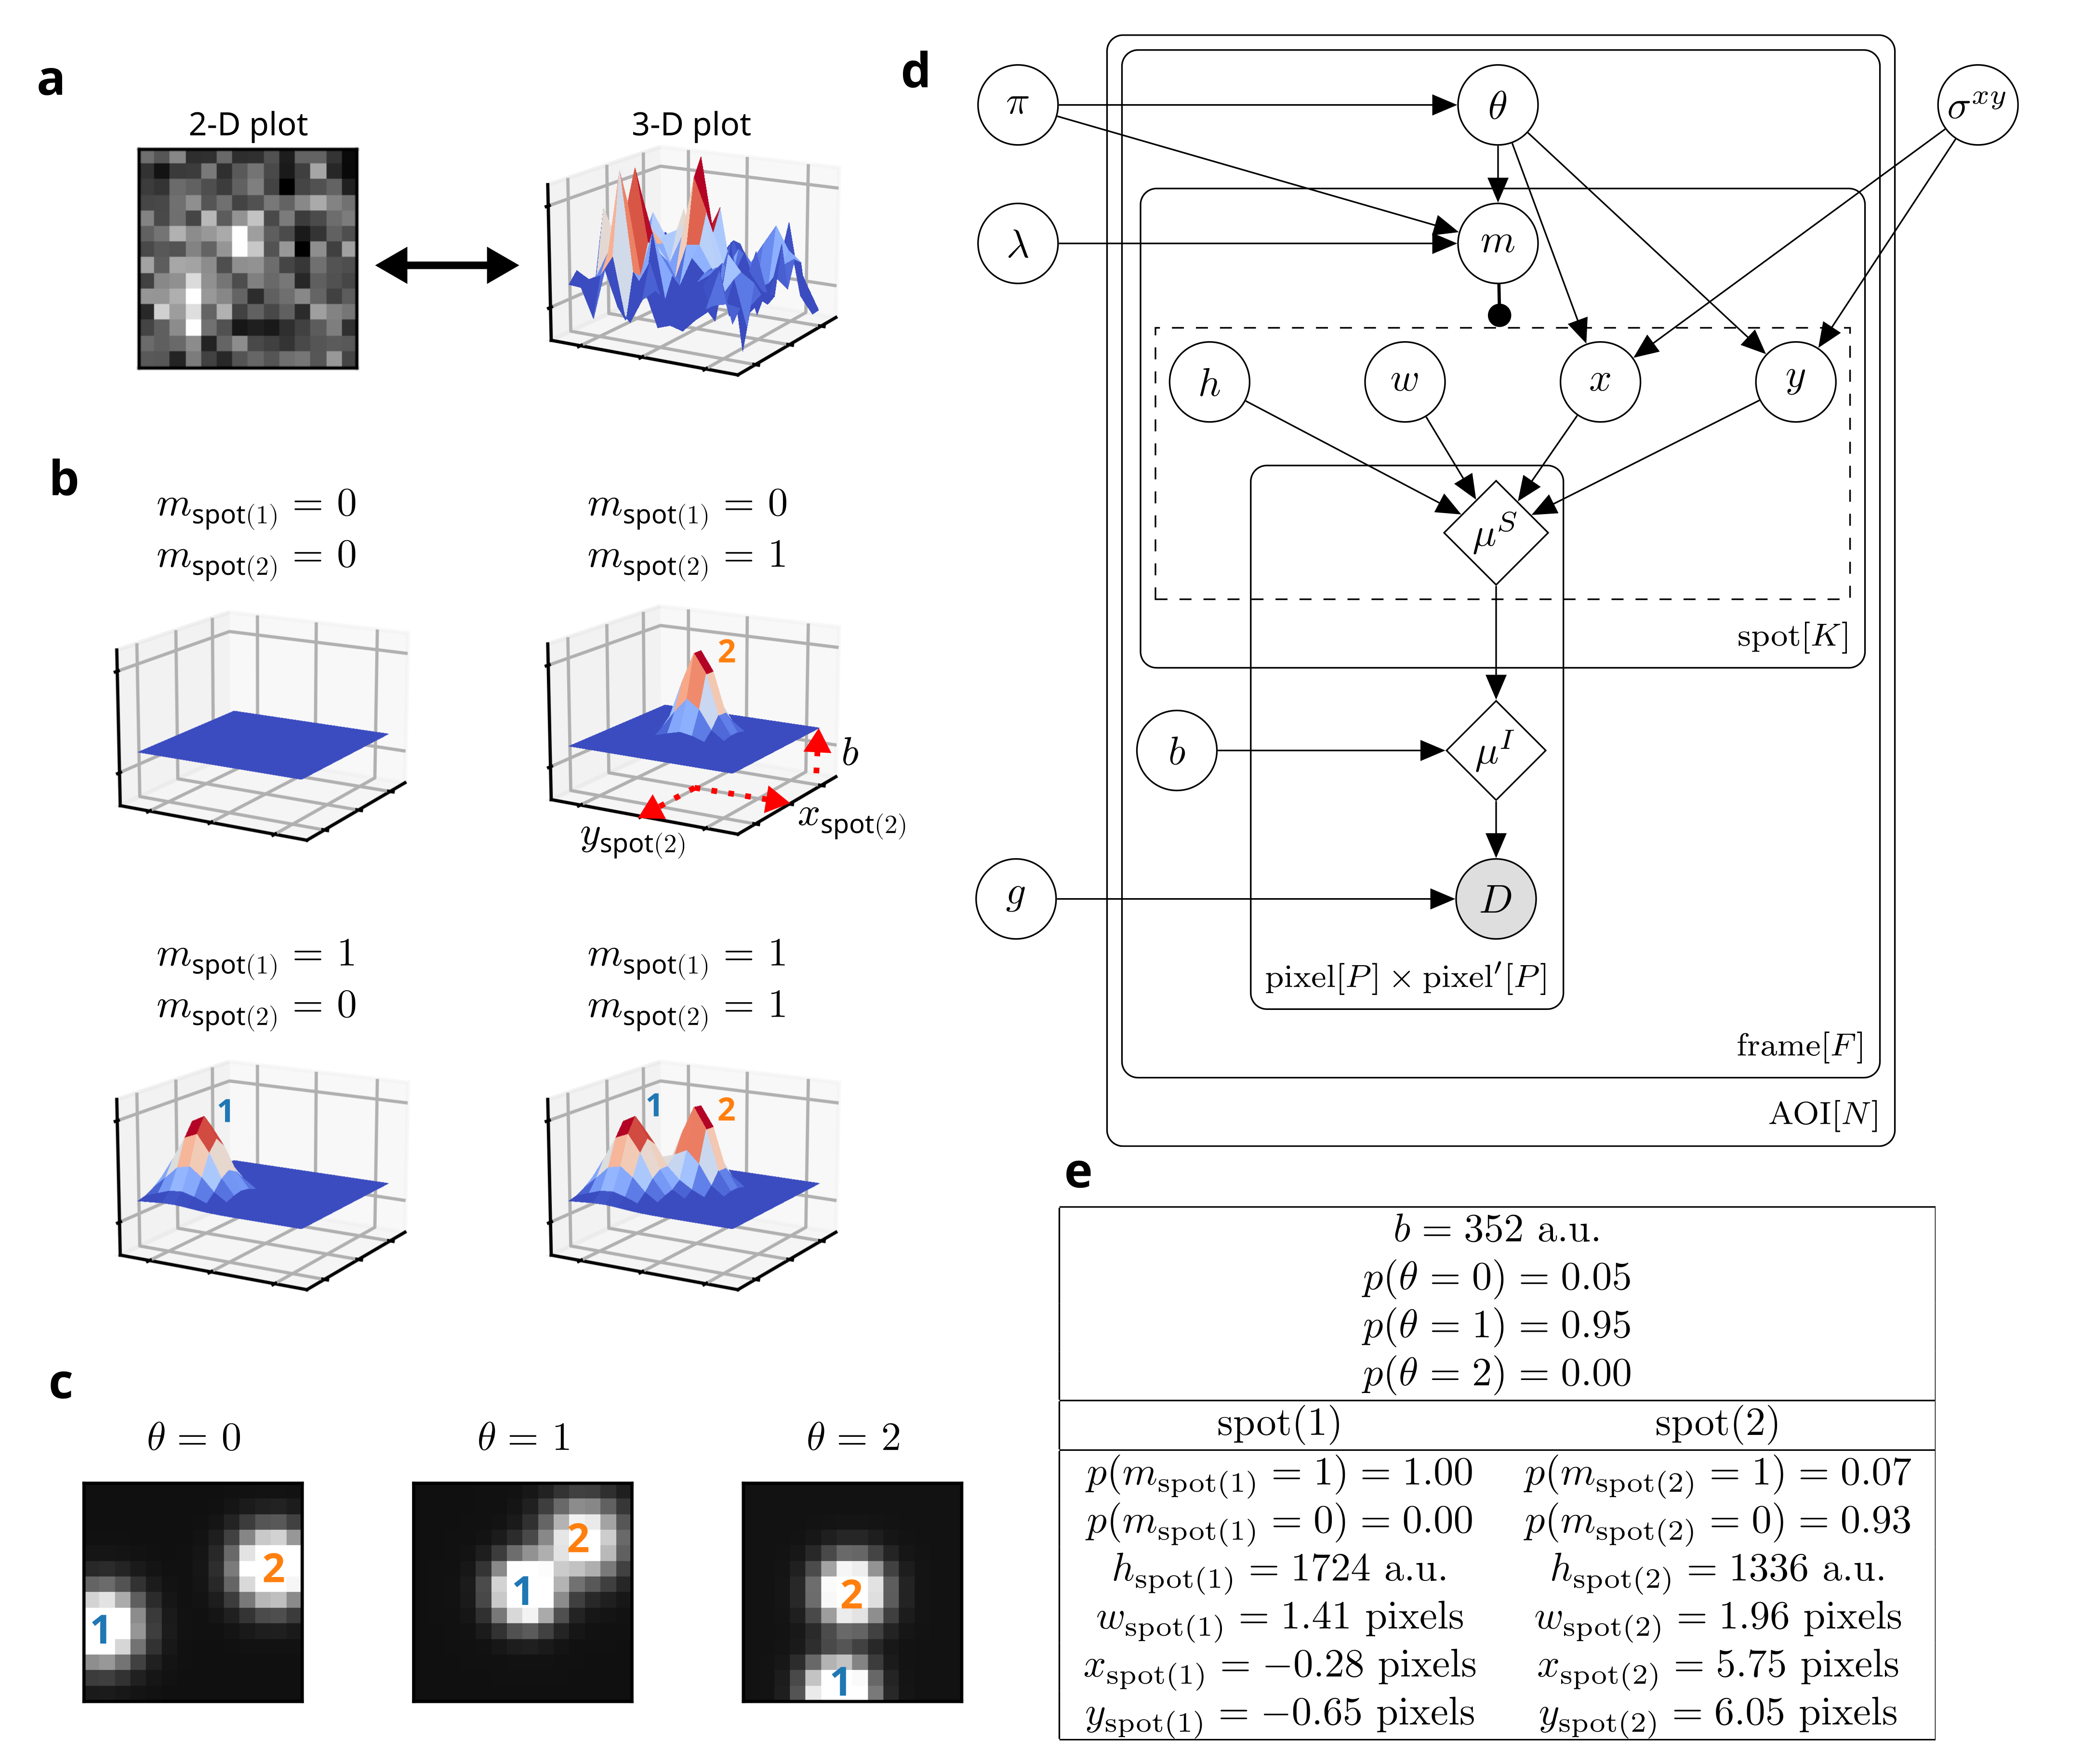
\includegraphics[width=\linewidth]{figures/figure2/figure2.png}
%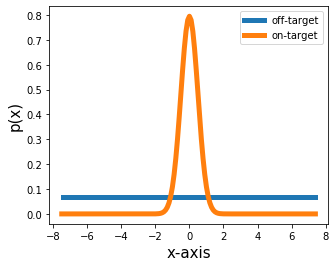
\includegraphics[width=\linewidth]{figures/figure2g.png}
\caption{Image models. CoSMoS images are modeled as 2D Gaussian spots superimposed onto the background intensity and the offset. Examples of the ideal image shapes for cases when there are (A,E,I) no spots, (B,F,J) single on-target spot, (C,G,K) single off-target spot, and (D,H,L) two spots. Noisy images (I-L) are generated using Gamma distribution with the parameter gain = 7 as described in the text.}
\label{fig:model}
\end{figure}

\subsubsection{Noise model}

\begin{comment}
Shot noise originates from a stochastic nature of photon counting which can be modeled by a Poisson process. The number of photons that fall on each pixel of the camera is Poisson distributed where the variance of the signal equals the mean value of the signal. Gain is a camera setting that amplifies the signal from camera sensors. Our model uses Gamma distribution parameterized by mean intensity ($\mu^D_{nfij}$) and gain ($g$) to model the linear relationship between the expected value of the signal and the variance with which the signal scatter about its expected value. Figure \ref{fig:model}  shows images  where the ideal images were perturbed with Gamma noise for no-spot (D), single spot (E), and two spots (F) images.
\end{comment}

Observed images are contaminated by noise. Noise is a stochastic phenomenon and therefore is described by the likelihood function. The likelihood describes the probability of the observed image given the image model. Scatter about the expected value of signal intensity ($\mu^I_{nfij}$) is determined by photon shot noise and the camera gain that amplifies the signal. We use Gamma distribution as a noise model which is more flexible than Gaussian noise and can better approximate Poissonian camera noise. In addition, there is a noise in the offset signal. Its distribution can be obtained from the camera images:

\begin{equation}
    I_{nfij} \sim \textbf{Gamma} (\mu^I_{nfij}, \sqrt{\mu^I_{nfij} \gamma})
\end{equation}

\begin{equation}
    \delta_{nfij} \sim \textbf{Categorical}_{\{ \delta_r \}^R_{r=1}}(\bm{\pi}^\delta)
\end{equation}

\begin{equation}
    D_{nfij} = \delta_{nfij} + I_{nfij}
\end{equation}

where $I_{nfij}$ is the signal intensity and $\gamma$ is the gain setting of the camera. $\delta_{nfij}$ is a camera offset and $\bm{\pi}^\delta$ is its distribution that can be obtained empirically from the dark corners of the images.

\subsubsection{Priors}
Prior distribution describe our assumptions about the model. On-target spots have a Bernoulli distribution with average probability $\pi^z$, while the number of off-target spots has a truncated Poisson distribution with the rate parameter $\lambda^j$. For the spot intensity we assume broad range of values given by:

\begin{equation}
    h_{knf} \sim \mathbf{HalfNormal}(\sigma^h)
\end{equation}
 
 Spot width has a uniform prior confined to a range:
 
\begin{equation}
    w_{knf} \sim \textbf{Uniform}(w_{\min}, w_{\max})
\end{equation}

Priors for the position of the spot depends whether the spot is on-target or non-specific. On-target spots are localized around the target molecule within the experimentally determined co-localization accuracy. On the other hand, non-specific binding can occur anywhere within the image and therefore has a uniform distribution across the image:

\begin{equation}
    x_{knf}, y_{knf} \sim
    \begin{cases}
    \textbf{AffineBeta}(0, \nu^{xy}, -\frac{P+1}{2}, \frac{P+1}{2}) & \text{$\theta_{nf} = k$ (on-target)} \\
    \textbf{Uniform}(-\frac{P+1}{2}, \frac{P+1}{2}) & \text{$\theta_{nf} \neq k$ (off-target)}
    \end{cases}
\end{equation}

Due to the irregularity of the filed of view of the microscope we assume separate prior for each target site:

\begin{equation}
    b_{nf} \sim \textbf{Gamma}(\mu^b_n, \sigma^b_n)
\end{equation}

\begin{table}
\caption{\label{tab:states}State space for $K = 2$.}
% Use "S" column identifier to align on decimal point 
\begin{tabular}{c c c c c}
\toprule
state   & first spot $m_{nf1}$ & second spot $m_{nf2}$ & on-target index $\theta_{nf}$  & probability \\
\midrule
$1$       & $0$     & $0$     & $0$         &  \\
$2$       & $1$     & $0$     & $0$         &  \\
$3$       & $0$     & $1$     & $0$         &  \\
$4$       & $1$     & $1$     & $0$         &  \\
$5$       & $\mathbf{1}$    & $0$     & $1$         &  \\
$6$       & $\mathbf{1}$    & $1$     & $1$         &  \\
$7$       & $0$     & $\mathbf{1}$    & $2$         &  \\
$8$       & $1$     & $\mathbf{1}$    & $2$         &  \\
\bottomrule
\end{tabular}
\end{table}

\subsubsection{Joint Distribution}

Factorization of the joint probability of the model is given by:

\begin{equation}
    p_\psi (\mathbf{D}, \mathbf{v})
    = p_\gamma (\mathbf{D} | \mathbf{b}, \mathbf{m}, \mathbf{h}, \mathbf{w}, \mathbf{x}, \mathbf{y})
    p_{\mu^b, \sigma^b} (\mathbf{b})
    p (\mathbf{h})^\mathbf{m}
    p (\mathbf{w})^\mathbf{m}
    p_{\sigma^{\mathrm{xy}}} (\mathbf{x}|\mathbf{\theta})^\mathbf{m}
    p_{\sigma^{\mathrm{xy}}} (\mathbf{y}|\mathbf{\theta})^\mathbf{m}
    p_{\pi^z, \lambda^j} (\mathbf{m}, \theta)
\end{equation} 

where $\psi = \{ \pi^z, \lambda^j, \mu^b, \sigma^b, \gamma \}$ and $\mathbf{v} = \{ \mathbf{b}, \mathbf{m}, \theta, \mathbf{h}, \mathbf{w}, \mathbf{x}, \mathbf{y} \}$.

\subsection{Inference}

The evidence, i.e. probability of the data, is given by:

\begin{equation}
    p_\psi (\mathbf{D}) = \int_\mathbf{v} p_\psi (\mathbf{D}, \mathbf{v}) d\mathbf{v}
\end{equation}

Our goal is to learn good model parameters by maximizing the log evidence:

\begin{equation}
    \psi_{\max} = \argmax_\psi \log p_\psi (\mathbf{D})
\end{equation}

In addition, we want to obtain the posterior over the latent variables $\mathbf{v}$ given the observed data:

\begin{equation}
    p_{\psi_{\max}} (\mathbf{b}, \mathbf{m}, \theta, \mathbf{h}, \mathbf{w}, \mathbf{x}, \mathbf{y}|\mathbf{D}) =
    \dfrac{p_{\psi_{\max}}(\mathbf{D}, \mathbf{b}, \mathbf{m}, \theta, \mathbf{h}, \mathbf{w}, \mathbf{x}, \mathbf{y})}
    {\int_{\mathbf{b}, \mathbf{h}, \mathbf{w}, \mathbf{x}, \mathbf{y}}
    \sum_{\mathbf{m}, \theta}
    p_{\psi_{\max}} (\mathbf{D}, \mathbf{b}, \mathbf{m}, \theta, \mathbf{h}, \mathbf{w}, \mathbf{x}, \mathbf{y})
    d\mathbf{b} d\mathbf{h} d\mathbf{w} d\mathbf{x} d\mathbf{y}}
\end{equation}

\begin{equation}
    p_{\psi_{\max}}(\mathbf{b}, \mathbf{m}, \theta, \mathbf{h}, \mathbf{w}, \mathbf{x}, \mathbf{y}|\mathbf{D})
    \simeq q_{\phi}(\mathbf{b}) q(\mathbf{m}, \theta) q(\mathbf{h})^\mathbf{m}
    q(\mathbf{w})^\mathbf{m} q(\mathbf{x})^\mathbf{m} q(\mathbf{y})^\mathbf{m}
\end{equation}

\subsection{Experimental data}

In this experiment, we labeled the NusG protein with an orange dye. We then tethered to a microscope slide blue-dye-labeled DNA molecules at very low surface density (so that each molecule is resolved as a separate fluorescent spot) and observed real-time binding and dissociation of the other labeled molecules during the transcription process and its regulation. The signal from the orange dye was split between short wavelength and long wavelength channels. The signal in the short wavelength channel was attenuated to varying degree to produce data sets with a range of SNR. Images from the long wavelength channel with high SNR were analyzed to determine "true" identities of the images.

%\subsection{Image analysis, probabilities not binary classification}

%Expresses uncertainty. Allows downstream analysis. 

%\subsection{Flexible framework. Can select and use different models depending on the experiment}

%\subsubsection{Ability to jointly analyze different experimental conditions}

%\subsubsection{Models easily expandable to incorporate other data features}
